\documentclass[main.tex]{subfiles} 
\begin{document}

\section*{Resultater \& Drøfting}
\label{sec:4}

%Når elever skal vurderes så kan dette gjøres på flere måter:
%\begin{itemize}
%\item Normalfordeling og fast poengsum : da blir vurderingsgrunnlaget \emph{de andre elevenes prestasjoner}. 
%Dette blir også referert som relativ vurdering. Vurdering av en individ avhenger da av de andre
%elevenes prestasjoner. Ved fast poengsum innebærer det at det er etter poeng oppnåelse elevene blir vurdert. 
%Da vil karakterene avgjøres ut ifra hvor mye peongsum eleven har klart å oppnå. Her vil ofte vanskelig oppgaver
%bli vektlagt mer enn enkelere oppgaver.
%\item Individrelatert kriterier : da vurderes eleven utelukkende i forhold til sine egne forutsetninger
%og tidligere prestasjoner. I grunnskolen skal vurderingen uten karakterer i hovedsak være 
%individrelatert  (\citeNP[s. 25]{hell07}).
%\item Målrelatert kriterier : kvalitetsstandarden blir da en didaktisk kontretisering av kompetansemål.
% I grunnskolen skal vurderingen med karakterer skje etter målrelaterte kriterier (\citeNP[s. 26]{hell07}).
%\item Kompetansemål : da vurderes elevene utfra hvilket nivå eller trinn (i henhold til Bloom's taksonomi) 
%                      de demonstrer i sin oppnåelse av kompetansemålene.
%\end{itemize}
%Jeg er nok enig i at bruken av individrelatert vurdering er en god vurderingsgrunnlag i situasjoner
%der karakterer ikke brukes. Denne vurderingsformen oppfyller kriterier for god vurdering, siden den brukes til å 
%fortelle eleven hvor hen befinner seg i sin faglig progresjon. Når lærer og elev sammen setter individuelle mål, både 
%nærliggende og langsikte, da vil eleven gjennom et slikt vurderingsgrunnlag få konkete tilbakemeldinger og 
%fremovermeldinger som fokuserer på nettopp elevens prestasjoner og målsettinger som hen har laget sammen med
%læreren (\citeNP[s. 200]{olma15}). Det kan også være fordelsaktig å koble målsettingene til kompetansenivå eleven 
%demonstrerer og jobbe mot høyre kompetansenivå. For eksempel diskutere er et høyt kompetansenivå, der eleven 
%kan trekke sammnenhenger og redegjøre for sine tanker om en problemstilling. I motsetning er å beskrive et middels 
%kompetansenivå (i Bloom's taksonomi).

Ved kartlegging av elevenes svakheter og styrker, er det da passende å bruke
individrelaterte kritier (\citeNP[s. 25]{hell07}) og koble inn kompetansemålene. Til en kartleggingsprøve så er det 
vanskelig å trekke inn individrelaterte kriterier med mindre lærer har godt kjennskap til eleven på forhånd. Jeg 
koblet dessverre ikke inn kompetansemålene heller, noe som det bør brukes mer av. Gjennom noen av mine samtaler 
med elever, oppdaget jeg fort at det var få som trakk forbindelsen mellom egen læring og koblingen til kompetansemålene. 
For undervisere regnes det som en god praksis at elevene er alltid bevisste om hvorfor de lærer det de lærer og hvor 
de er på vei. \citeA[s. 136]{klet13} beskriver en god undervisningsseksens der lærere klarer å balansere mellom 
tilegnelses-, utprøvings-, og konsolideringssituasjoner. Ifølge Klette har norske klasserom ensidige tendenser i bruken 
av varierte arbeidsmåter. Slik det kan ses fra figur \ref{fig:odeg10}, er det for eksempel lite 
konsolideringssituasjoner. Lærernes metalæringsaktiviteter regnes som særlig avgjørende for å sikre elevenes læring 
(\citeNP[s. 186]{klet13}). Å bruke dette som et fast organiserende prinsipp, blir derimot sjelden gjennomført 
(\citeNP[s. 26]{odeg10}).
\begin{figure}[h!]
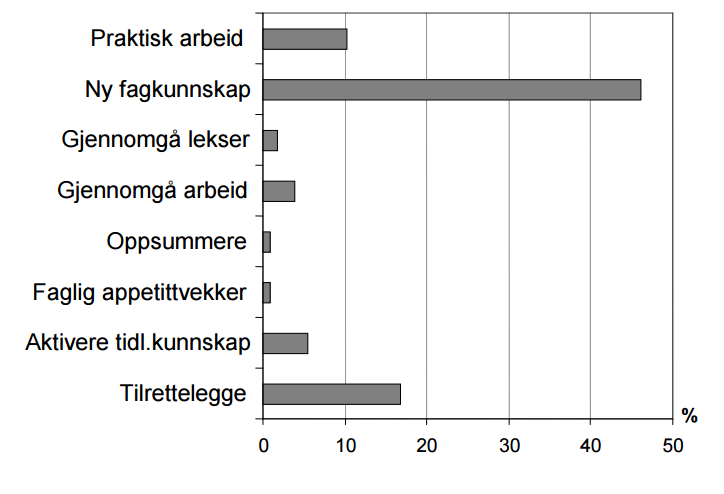
\includegraphics[scale = 0.6]{../figures/undervisnings_aktivitet.png}
\caption{Oversikt over naturfaglærernes undervisningstilbud til elevene fra PISA+ studie. Kilde: 
\protect\citeA{odeg10}.}
\label{fig:odeg10}
\end{figure}
\newline

Før resultatene til kartleggingsprøven var jeg informert av min veileder om at klassens snitt lå et sted mellom
karakter 2 og 3. Dermed forventet jeg også at elevene ville prestere lavt på kartleggingsprøven. På figur 
\ref{fig:scoreoversikt} kan vi se at mange elever ligger under en score på 4 ut av 10, med en gjennomsnitt 
på circa 3. Det var 2 blanke besvarelser og 7 av 27 elever var ikke til stede.
\begin{figure}[h!]
\centering
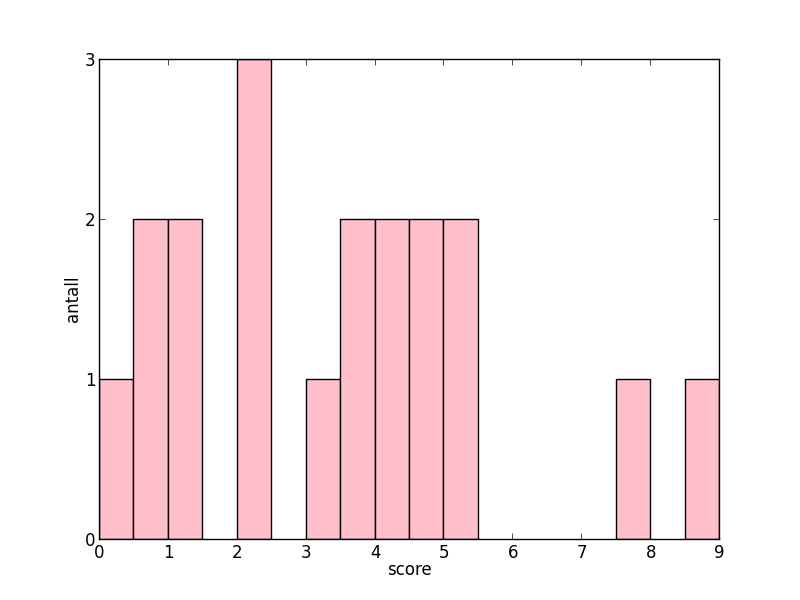
\includegraphics[scale = 0.5]{../figures/scoreoversikt.png}
\caption{Resultater fra kartleggingsprøven - Oversikt over score}
\label{fig:scoreoversikt}
\end{figure}

Det var på forhånd avtalt med elevene at kartleggingsprøven var ikke en del av summativ vurdering, men skulle brukes
som den del av formativ vurdering. Derimot, siden jeg hadde ikke valgt å gi elevene enn slutt vurdering, annet enn en 
poengsum, hadde det en mulig uheldig effekt. Fra mine observasjoner og samtaler med elevene kom det frem at noen av 
elevene anstrengte ikke like hardt som de ellers ville ha gjort hvis kartleggingsprøven var en ``virkelig'' prøve.
Gjennom elevsamtale med en av de sterke elevene, spurte jeg eleven hvorfor hen ikke hadde besvart en spesifikk 
oppgave og eleven svarte med å si at oppgaven var lett, men hen ``orket'' ikke å gå gjennom den. Grunnen hen oppga 
var at siden det ikke var en prøve, hadde det ikke så mye betyning. Dette samsvarer godt med det \citeA[s. 3]{brbl14} 
skriver : 
\begin{displayquote}
Vurdering kan ha en betydelig påvirkning på hvordan elever jobber, fordi de oppfatter det som 
vurderes som det eneste ``som teller''.
\end{displayquote}
Jeg hadde dessuten vektlagt de ``vanskelige'' oppgavene mye mer enn de ``enkle''. Nesten alle elever på tvers av nivå og 
ferdigheter hadde problemmer med å løse disse oppgavene og veldig få klarte å gå over en score på 5 ut av 10. Dermed 
fikk jeg ikke veldig mye informasjon om elevene gjennom poengsum. Ofte var det de over middelssterke elevene i klassen 
som tangerte mot 5 i poengsum. Kun en elev klarte å oppnå en score på 8.5. Det er verdt å merke at hvis dette var 
en prøve så ville det ha vært viktig å skape situasjoner der elever kan vise mestring (\citeNP[s. 199]{olma15}). 
Siden dette var en kartleggingsprøve var fokuset isteden rettet mot å avklare elevens misoppfattelser og få en oversikt 
over hvor elevene ligger i sin læringsprossess. Her vil jeg derfor påstå at det er viktig å gjøre et slikt skille, men 
det bør selvfølgelig skapes litt rom for å la elevene kjene på mestringsfølelsen. Dette vil jeg ta hensyn til videre i
mitt vurderingsarbeide. Videre nå vil jeg snakke om individuelle oppgaver fra kartleggingsprøven og diskutere 
elevenes feiltolninger.

\subsection*{Elevenes feiltolkninger}
Ifølge \citeA[s. 15]{brek02} og \citeA[s. 170]{olma15} kan diagnostiske oppgaver bli brukt til å identifisere og 
fremheve misoppfatninger som elevene har utviklet, gi læreren informasjon om elevenes løsningsstrategier og måle hvordan 
undervisningen har hjulpet elevene til å overvinne misoppfatningene. Gjennom blant annet kartleggingsprøver får elever 
muligheter til å utrykke sine skriftlige ferdigheter i matematikk. Å skrive matematikk regnes som en av grunnleggende 
ferdighetene. Det innebærer blant å beskrive og forklare egen tankgegang, å lage tegninger og skissere grafer. 
Skriving i matematikk blir sett på som et redskap for å utvikle egne tanker og egen læring (\citeNP{udirGF}). 

Pyskologene Daniel Kahneman og Amos Tversky har satt fram en teoretisk 
ramme for å undersøke læring av sannsynlighet og statistikk. Deres tese er at mennesker uten erfaring, refleksjon og 
innsikt i statistikk, bruker følgende strategier for å bedømme sannsynlighet (\citeNP{udir13}; \citeNP{evan17}):
\begin{itemize}
\item Representativitet : små utvalg skal representere den fordelingen som finnes i populasjonen
\item Tilgjengelighet : sannsynlighet bedømmes ut fra hvor lett det er å huske spesielle tilfeller
\item Resultatorientering : utfallet kan forutses, som ved en deterministisk prosess
\item Konjunksjonsfellen : sannsynligheten for at to hendelser inntreffer samtidig er mindre enn sannsynligheten
for at en av hendelsene inntreffer.
\item Generelt vanskeligheter med betinget sannsynlighet : dvs. vanskeligheter med sannsynligheter hvor et utfall
avhenger av foregående utfall. Imotsetning er ubetinget sannsynlighet utfall der en begivenhet forekommer uavhengig 
av tidligere utfall (se også vedlegg 2). 
\end{itemize}
Dette er ofte misoppfattelser som også ligger hos elever ved ulike faglignivå. For eksempel en vanlig feil
mange elever gjør er at de blander addisjonsregelen med muliplikasjonsregelen (se vedlegg 2). Det kan godt hende at dette
skyldes at de bruker eksempeler de husker gjennom informasjon de har tilgjengelig. F.eks. hvis en oppgave minner
dem om et tilfelle der de brukte addisjonsregelen, vil de prøve å bruke den, selv når situasjonen krever bruk
av multiplikasjonsregelen. Dette har jeg observert både gjennom undervisning av sannsynlighetsregning og
gjennom kartleggingsprøven (se figure : \ref{fig:mohsin}). Gjennom praksis, i mitt forsøk med å rette disse 
misoppfattelser har vært å tydeliggjøre forskjellen mellom disse to reglene. 
\newline

\subsection*{Rom for tolkning blant elevenes misoppfattelser}
Det var en deloppgave i kartleggingsprøven som mange elever feiltolket (se figure \ref{fig:oppgave4}), og det er 
godt mulig å akseptere at oppgaveteksten kan tolkes på en annen måte enn tilsiktet.
\begin{figure}[h!]
\centering
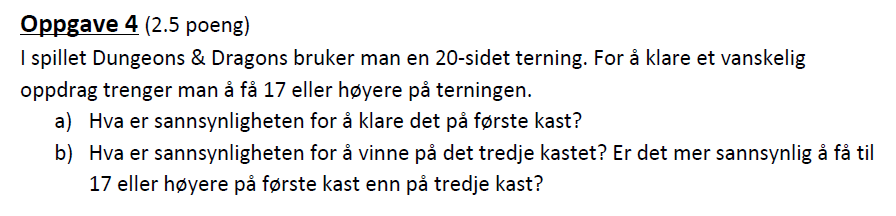
\includegraphics[scale = 0.6]{../figures/oppgave4b.png}
\caption{Oppgave 4}
\label{fig:oppgave4}
\end{figure}
I oppgave b står det \emph{Hva er sannsynligheten for å vinne på det tredje kastet?}. Her er hensikten at
at utfallet avhenger av to foregående utfall. Det vil si : \emph{Hva er sannsynligheten for å 
tape på to runder på rad og deretter vinne på det tredje kastet?}. Mange oppfattet det som å vinne på tredje kastet 
uavhengig av hva som forekommer på de første to kast. Dermed ville svaret til neste del av deloppgaven, \emph{Er det mer 
sannsynlig å få til 17 eller høyere på første kast enn på det tredje kast?},  være ``like sannsynlig'' og det var ofte 
det elevene besvarte. Tiltross for at en del av elevene svarte like sannsynlig, førte de opp sannsynligeter som 
ikke samsvarte med deloppgave 4.a. Dermed viste de at de hadde vansker med betinget sannsynlighet og at deres svar var 
valgt basert på feiloppfattelser om betinget sannsynlighetsregning. For eksempel i figur \ref{fig:maria} har eleven 
ganget svaret fra deloppgave a med 3 i både nevner og teller. Tiltross for at eleven tror at svaret skal være samme som 
i deloppgave a, forsøker eleven å manipulere uttrykket. Etter å ha snakket muntlig med eleven viste det seg at eleven 
tenkte at siden sannsynligheten befinner seg i tredje trinn i utfallstreet, så er det tilstrekkelig å gange svaret fra 
deloppgave a med 3 i teller og nevner. Her var det flere ting som kom fram som viste at eleven hadde både problemmer
med betinget sannsynlighet men også tallforståelse. Dette ble også lagt merke til fra elevens besvarelse i deloppgave 3 
b. Derimot var det lovende at eleven kunne visualisere for seg at hvor sannsynligheten befant seg i utfallstreet. 
\begin{figure}[h!]
\centering
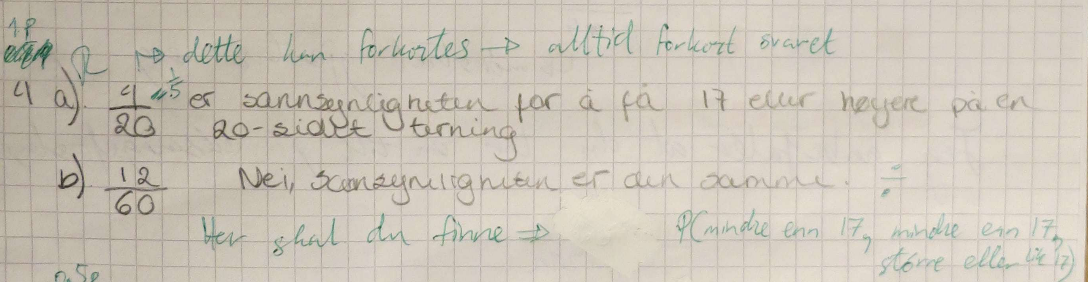
\includegraphics[scale = 0.3]{../figures/maria.png}
\caption{Oppgave 4}
\label{fig:maria}
\end{figure}

I oppgave 4.b har elevene anledning til å demonstrere høyt kompetansenivå. Dessverre er formuleringen ikke
godt nok til å trekke elevene inn i et diskurs. Her burde det gjerne ha blitt lagt til en bisetning, som 
for eksempel \emph{``Kan du gi en forklaring?''}. Med slike spørsmål er det lettere å oppdage elevenes
feiltolkninger, fordi da slipper en å få besvarelser som er enten ``ja'' eller ``nei''. Oppgave 
5.b var bedre formulert (se vedlegg 1). Her kreves det eksplisitt en forklaring fra elevene.
Dette er en fin øvelse for elever å demonstrere at de har forstått bruken av utfallstreet. Det var derimot
få elever som fikk til oppgaven, og enda fære som prøvde å gi en forklaring. Etter å snakket med elevene
som forsøkte å løse oppgaven, var forklaringen deres at enten så overså de krav om begrunnelsen, eller de var
ikke sikker på forklaringen. De som overså krav om begrunnelsen, neglisjerte denne delen av oppgaven fordi
de fikk ikke med seg at det skulle legges til en forklaring, og de andre svarte at en forklaring var ikke
viktig å få med.

\begin{figure}[h]
\centering
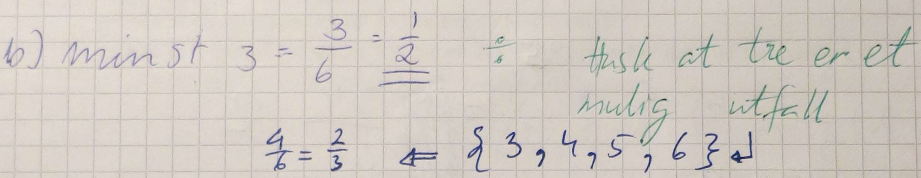
\includegraphics[scale = 0.4]{../figures/maryam.png}
\caption{Oppgave 1}
\label{fig:maryam}
\end{figure}

\subsection*{Tilbakemeldinger}

William redegjør for hvorfor tilbakemeldinger noen ganger kan føre til senking 
i elvenes ytelse. Han referer til Kluger og DeNisi (1996), når han summerer opp 
\begin{displayquote}
\textelp{} feedback was least effective when it focused on the task in hand, 
and more effective when it focused on the details at hand, and most effective 
when it focused on the details of the task and involved goal-setting.
(\citeNP[s. 140]{will10})
\end{displayquote}

\begin{figure}[h!]
\centering
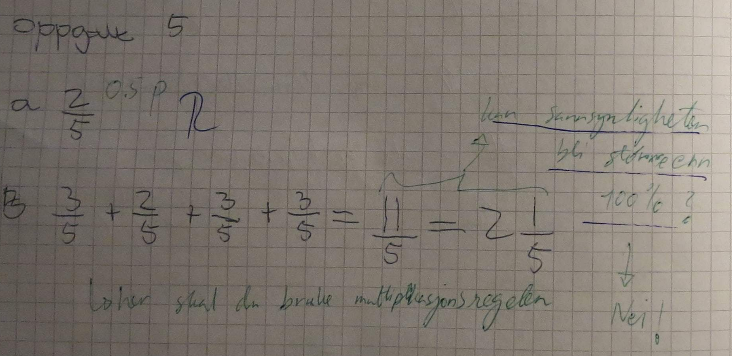
\includegraphics[scale = 0.4]{../figures/mohsin.png}
\caption{Oppgave 5}
\label{fig:mohsin}
\end{figure}

I figur \ref{fig:mohsin2} har jeg gitt en tilbakemelding som fokuserer på
elevens besvarelse fra figure \ref{fig:mohsin}. I tilbakemeldingen er fokuset
rettet mot detaljene i oppgaven og veileder eleven videre til å rette sine
misoppfattelser. Her kan målene tydeliggjøres endatil.

\begin{figure}[h!]
\centering
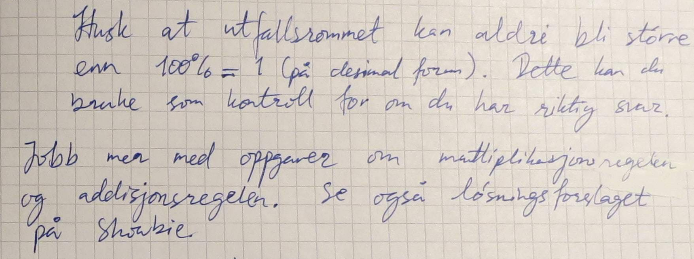
\includegraphics[scale = 0.4]{../figures/mohsin2.png}
\caption{Tilbakemelding og fremovermelding}
\label{fig:mohsin2}
\end{figure}

\end{document}
